\documentclass[oneside,12t]{classes/Thesis}

\usepackage[utf8]{inputenc}
\usepackage{ulem}
\usepackage[english]{babel}

\usepackage{url}
\graphicspath{{img/}}
\DeclareGraphicsExtensions{.pdf,.png}

\usepackage{fixltx2e}


\usepackage{algorithm}
\usepackage{algorithmic}
\usepackage{caption}
\usepackage{subfigure}

\title{A task based programming model for the fine-grain parallelization of sparse linear solvers}


\authorFirstName{Corentin}
\authorLastName{Rossignon}
\authorMail{corentin.rossignon@gmail.com}

\directors{Pascal \textsc{H\'{e}non}, Olivier \textsc{Aumage}, Samuel \textsc{Thibault} and Raymond \textsc{Namyst}}

\laboratory{LaBRI}
\laboratoryURL{http://www.labri.fr/}
\university{Université de Bordeaux}
\universityURL{http://www.univ-bordeaux.fr/}


\logo{bordeaux1}
\degreeDate{??th ???? 201?}
\degree{Doctor in Computer Science}
\degreeSpeciality{High Performance Computing}

\metadataSetup

% turn of those nasty overfull and underfull hboxes
\hbadness=10000
\hfuzz=50pt

\begin{document}

\dominitoc
\tikzstyle{decision} = [diamond, draw, fill=blue!20,
text width=3em, text centered, node distance=2.5cm, inner sep=0pt,font=\scriptsize]
\tikzstyle{block} = [rectangle, draw, fill=blue!20,
text width=4em, text centered, rounded corners, minimum height=1em,font=\scriptsize]
\tikzstyle{line} = [draw, thick, color=black!50,font=\scriptsize]
\tikzstyle{cloud} = [draw, ellipse,fill=red!20, node distance=2.5cm,
minimum height=0.1em,font=\scriptsize]

\maketitle

%set the number of sectioning levels that get number and appear in the contents
\setcounter{secnumdepth}{3}
\setcounter{tocdepth}{3}

\frontmatter % book mode only
\pagenumbering{roman}
%Test

%La résolution de grands systèmes linéaire creux est un élément essentiel des simulations numériques. Ces résolutions peuvent représenter jusqu'à 80\% du temps de calcul des simulations.
Une parallélisation efficace des noyaux d'algèbre linéaire creuse conduira donc à obtenir de meilleurs performances. En mémoire distribuée, la parallélisation de ces noyaux se fait le plus souvent en modifiant le schéma numérique. Par contre, en mémoire partagée, un parallélisme plus efficace peut être utilisé. Il est donc important d'utiliser deux niveaux de parallélisme, un premier niveau entre les noeuds d'une grappe de serveur et une deuxième niveau à l'intérieur du noeud. Lors de l'utilisation de méthodes itératives en mémoire partagée, les graphes de tâches permettent de décrire naturellement le parallélisme en prenant comme granularité le travail sur une ligne de la matrice. Malheureusement, cette granularité est trop fine et ne permet pas d'obtenir de bonnes performances.
Dans cette thèse, nous allons étudier le problème de la granularité pour la parallélisation par graphe de tâches. Nous proposerons d'augmenter la granularité des tâches de calcul en créant des agrégats de tâches qui deviendront eux-mêmes des tâches. L'ensemble de ces agrégats et des nouvelles dépendances entre les agrégats formera un graphe de granularité plus grossière. Ce graphe sera ensuite utilisé par un ordonnanceur de tâches pour obtenir de meilleurs résultats. Nous utiliserons comme exemple la factorisation ILU d'une matrice et nous montrerons les améliorations apportées par cette méthode. Dans un second temps, nous nous concentrerons sur les machines à architecture NUMA. Dans le cas de l'utilisation d'algorithmes limités par la bande passante mémoire, il est intéressant de réduire les effets NUMA liés à cette architecture. Nous montrerons comment prendre en compte ces effets dans un intergiciel à base de tâches pour améliorer les performances d'un programme.

Mots-clés : parallélisme, graphe de tâches, supports d’exécution, NUMA, multi-coeurs, algèbre linéaire creuse

%With the commoditization of multi-core processors in clusters, the inter-node parallelism expressed by HPC applications needs to be complemented by a finer-grained parallelism that takes advantage of shared memory at the intra-node level.
%
The fine grain parallelism means that we can exhibit new levels of parallelism by parallelizing some operations that are usually done sequentially.
%
Usually it consists in parallelizing some algorithms performed inside a MPI process by using several cores of a cluster node.
%
Indeed, by taking advantage of the shared memory at the node level, some algorithms are then parallelizable, whereas they could not be efficiently parallelized using the static partitioning of data and communication overhead imposed by a distributed memory framework (e.g., MPI).


Some popular shared memory parallel frameworks like Intel TBB~\cite{Intel::TBB},
Cilk~\cite{cilk} or OpenMP 3.0~\cite{openmp08} propose programming models that
considerably alleviate the fine grain parallelization in a shared memory environment.
Those models rely on the use of a scheduler that dispatches the computation tasks
at runtime on the available cores of a cluster node. The simplest form of fine grain
parallelism consists in splitting independent works done in a loop among the cores.
More complex algorithms require to expose the parallelism as an Direct Acyclic Graph (DAG)
where each node is a task that consists in a group of operations that
can only be computed once all its predecessor tasks have also been completed.
With such a computational task graph approach, the work that belongs to the developer
is to describe the computations as a collection of tasks and to give  the set of
predecessor and successor tasks for each of them. The runtime scheduler is then
in charge of launching tasks on the hardware and achieve a good load-balancing.

Nevertheless, these programming models lack some features to handle efficiently
some important classes of problems.
Indeed, very often two crucial problems have to be addressed in order to achieve
an efficient fine grain parallelization:
\begin{itemize}
\item The first one is to obtain a correct task grain size for a good parallel
  efficiency: A too fine parallelism grain leads to bad performances caused by
  the task management and scheduling overhead, while a too coarse grain does not
  provide enough parallelism for the hardware capability and causes load balancing issues.
\item The second problem is to take into account the Non Uniform Memory Accesses (NUMA)
  that are caused by the time penalty when a core needs to access some data that
  are not physically located on a memory bank directly linked to its socket.
  Therefore, the physical location of memory allocation needs to be carefully driven
  to match the task scheduler policy in order to minimize these time penalties.
\end{itemize}

In this paper, we present some solutions to address these two problems at the
level of the programming model.
Our main motivation is that we want a programming model that adds as few
programming effort as possible beyond a natural task based parallelization of
an algorithm (using TBB for example) to obtain a better efficiency by taking
care of NUMA and task grain size.

%%  To reach this goal, in the first place we have enhanced the C++ programming interface proposed by Intel TBB to
%%   add some coarsening operators based on the task description of a problem. To that end we have implemented a task aggregation library that does
%%   the coarsening graph operations using different heuristics that can be selected and combined by the user using a simple string parameter.
%%  % It is important to note that the default aggregation operator when merging two task consists in sequentially calling the function of each task in the coarse task
%%  % but a developer can also overload the aggregate operator of the task class to redefine how to merge two tasks; for example instead of calling sequentially each task function
%% %The coarsen graph obtained can then be used on top of any runtime scheduler: our implementation interface allow to use TBB, OpenMP or our own NUMA-aware scheduler
%%   %in a seamless manner; we can switch between runtime systems by simply adding a flag at compilation.
%%   We have interfaced this library with several runtimes (Intel TBB, OpenMP and also our own implementation of a runtime scheduler) that can execute the coarse task graph obtained after this steps.
%%   The second part of the work was to take care of NUMA effects. Our approach has been to provide some special allocators to the user so that

%To evaluate the benefit of our work we present some experiments on the
%parallelization of an iterative solver for sparse linear systems. A popular
%approach to solve large sparse linear systems of equations is a Krylov
%method (such as GMRES or Conjugate Gradient) preconditioned by an incomplete
%factorization (see~\cite{Saad96IMSLS}).
%This is often the most time consuming part of a numerical simulation.
%The usual way to parallelize this kind of solvers is to use a weaker form of
%the preconditioner in parallel by preconditioning subdiagonal blocks of the
%matrix: The subdiagonal blocks are usually obtained thank to a partition of
%the adjacency graph of the matrix.
%Outside the preconditioner, the operations required in a Krylov method are
%vector operations (mostly BLAS1 type like dot products or AXPY) and matrix % CR: CHECK: replace `,' by or
%vector products. Those operations are naturally dealt with parallel loop
%splitting  (e.g., {\em parallel for} in OpenMP).
%In this paper, we have chosen to focus on the fine grain parallelization of
%the ILU preconditioner.
%In this case, more levels of parallelism can be obtained because the factorization
%and triangular solves of a submatrix can be parallelized on several cores.
%Incomplete factorization and associated triangular solve of a sparse matrix
%is a problem that is well representative of the difficulty that one can encounter
%with fine-grain parallelization: The fine grain description of these algorithms
%is natural. However, in practice a straight task based parallelization using TBB or
%OpenMP does not deliver good speed-ups because of the very low computational cost of
%a task and the NUMA effect when accessing the coefficients of the matrix and vector.
%In the experiment results, we will evaluate our programming model on those algorithms.

%%   In a Krylov method the operation needed are vector operations (dot product, AXPY as define by BLAS1..) and matrix vector multiplications (the matrix
%%   is usually really sparse). The most complicated part for a fine grain parallelization
%%   We have specifically studied the parallelization of an incomplete LU factorization () and the triangular solves associated.

%%   LU
%%   (ILU(k)) factorization. The ILU factorization is a very popular preconditioner for Krylov met
%%   A very popular approach to solve linear system is a Krylov method like GMRES

%%   To handle the task grain problem our approach is to coarsen the fine-grained parallelism through
%%   general heuristics of graph coarsening based on the task graph description of the user. The originality
%%   of our approach is to alleviate the programming task by letting the developer express the natural task decomposition of its problem
%%   but then propose a simple operator of coarsening that will apply some heuristics to produce a coarsest task graph.

%%   application programmer first expresses the fine parallelism sparse
%%   linear algebra parallelism in a natural way. Then, our coarsening
%%   mechanism applies a selectable coarsening scheme to aggregate
%%   individual tasks as larger task groups, so as to efficiently feed the
%%   platform computing units.



%%   Sparse linear solvers are often the main computational bottleneck in numerical simulations; a large class of the iterative method are composed
%%   of a Krylov method preconditioned by an Incomplete LU (ILU) factorization (see for example).

%% %%   For sparse linear algebra computations, it is common to use domain
%% %%   decomposition to generate parallelism. In the special case of
%% %%   iterative methods, however, domain decomposition may impact the
%% %%   numerical stability and thus the number of steps required for reaching
%% %%   convergence. Moreover, the natural parallelism at the sparse linear
%% %%   algebra computation is too fine grained.

\tableofcontents
\mtcaddchapter
\mainmatter % book mode only



%=========================================================
\chapter{Context : Simulate petroleum extraction}
\minitoc
\vspace{1cm}
%=========================================================

%+++++++++++++++++++++++++++++++
\section{Reservoir simulation}
%-------------------------------
\subsection{Vue d'ensemble}
Dans les profondeurs de la Terre, du pétrole et du gaz naturel se trouvent piégés.
%
Ces sources d'énergie sont le résultat de la transformation de matière organique, provenant de végétaux et d'animaux morts, sous très fortes contraintes durant des millions d'années.
%
Les compagnies pétrolières telles que Total ont pour but de localiser et d'optimiser l'extraction de ces ressources.

Plus généralement, nous appelons réservoir d'hydrocarbure, ou simplement réservoir, une concentration majeure de pétrole et/ou de gaz naturel sous le sol.
%
La première étape pour trouver un réservoir consiste à analyser le sous-sol avec des ondes acoustiques.
%
Ces ondes sont générées par des explosions pour les analyses sous la mer ou avec un camion sismique pour la surface de la Terre.
%
Ces ondes sont ensuite analysées avec des logiciels de modélisation basés sur les équations des ondes, les compagnies pétrolières peuvent ainsi obtenir une bonne représentation du sous-sol.
%
Après analyse de cette représentation, des puits d'explorations sont forés pour s'assurer de la présence de pétrole.
%
Quand un réservoir est trouvé, l'une des premières questions est : ``Est-il rentable d'exploiter ce réservoir ?''.
%
La simulation de réservoir est un des outils permettant de répondre à cette question.
%
En faisant une simulation de fluides en milieu poreux, les compagnies pétrolières peuvent obtenir une approximation de la quantité d'huile pouvant être récupérée.
%
Si l'exploitation du réservoir est rentable, les compagnies pétrolières commencent l'exploitation.

Mais il ne suffit pas de creuser et d'attendre que le pétrole jaillisse sous la forme d'un geyser comme nous pouvons le voir dans certains cartoons.
%
Les compagnies pétrolières doivent installer des puits.
%
Les puits peuvent être catégorisés en deux catégories majeures (Fig.~\ref{fig:wells}) :
%
\begin{itemize}
  \item les puits injecteurs, ce sont les puits qui augmentent la pression à l'intérieur du réservoir en injectant de la matière (eau, gaz(CO$_2$), polymère ...);
  \item les puits producteurs, ce sont les puits qui récupèrent l'huile, ils sont aussi essentiels au contrôle de la pression en produisant plus ou moins d'huile et de gaz.
\end{itemize}
%   (-_-)   %
\begin{figure}[!h]
  \centering
  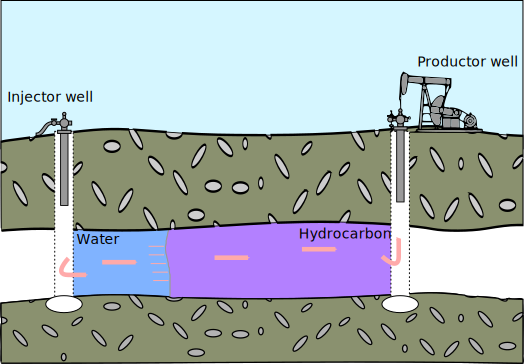
\includegraphics[width=0.8\textwidth]{wells}
  \caption{Exemple d'un champ avec deux puits.}
\label{fig:wells}
\end{figure}

L'une des activités des ingénieurs réservoir consiste à trouver le nombre optimal de puits ainsi que l'emplacement optimal de chacun pour exploiter le réservoir.
%
Encore une fois, la simulation de réservoir leur permet de tester différentes configurations de placement des puits.
%
Plus tard, quand la compagnie pétrolière commence à exploiter le champ, il est intéressant d'avoir des prévisions sur la production d'huile.
%
Une fois de plus, ces résultats sont obtenus avec une simulation de réservoir (Fig.~\ref{fig:floviz}).

%   (-_-)   %
\begin{figure}[!h]
  \centering
  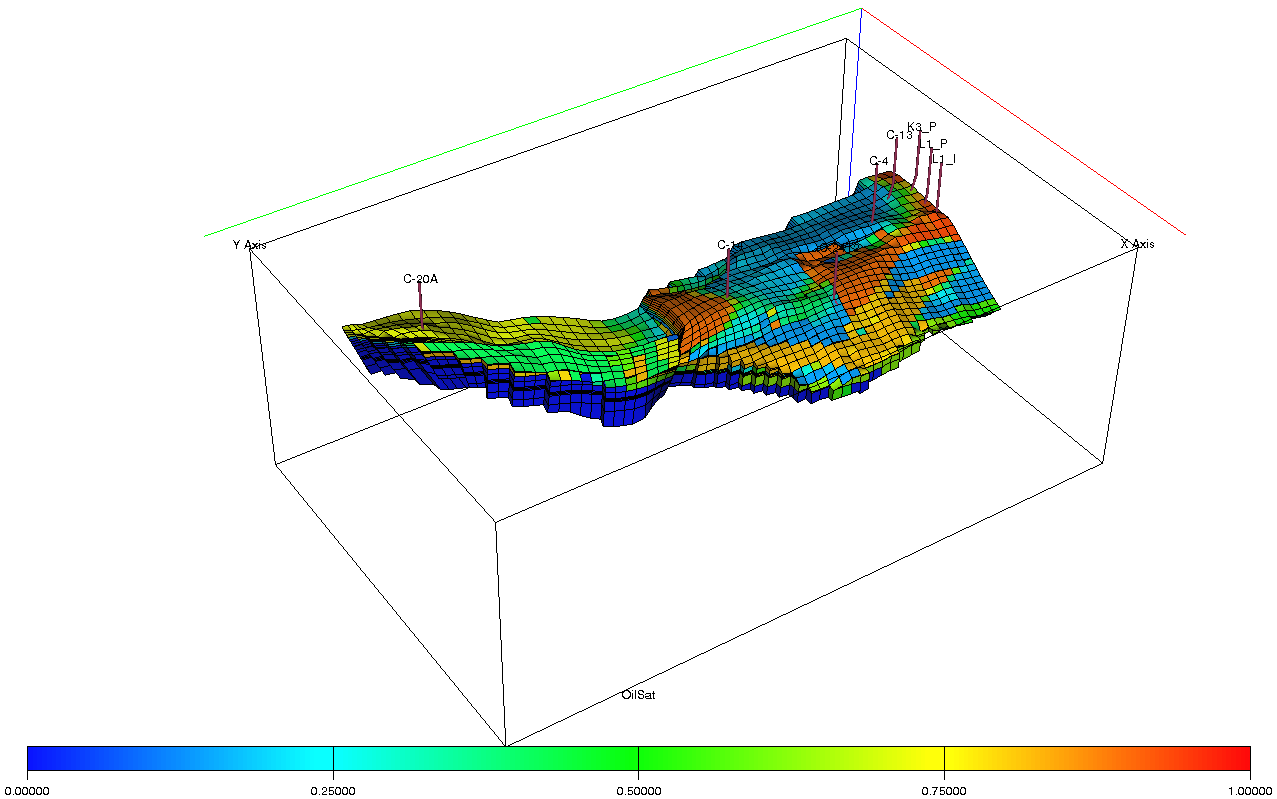
\includegraphics[width=\textwidth]{reservoir}
  \caption{Visualisation de la quantité d'huile dans le réservoir, l'image provient du logiciel floviz.}
\label{fig:floviz}
\end{figure}




Comme montré précédemment, la simulation de réservoir est une étape clé dans le processus de récupération d'hydrocarbures.
%
Il est intéressant pour une compagnie pétrolière de simuler de plus en plus précisément l'intérieur d'un réservoir et bien sûr le simuler aussi vite que possible.
%
Focalisons-nous sur la structure interne d'un simulateur de réservoir.

%-------------------------------
\subsection{De la physique au calcul informatique}
Pour pouvoir faire une simulation de réservoir, on démarre avec un physicien qui modélise un écoulement de fluide en milieu poreux.
%
La plupart de ces modèles sont basés sur trois équations physiques : la conservation de la masse, la loi des gaz parfaits et la loi de Darcy.
%
Puis le réservoir est discrétisé en cellules en utilisant la méthode des volumes finis.
%
Pour chaque cellule du réservoir, nous obtenons une équation non-linéaire par variables primaires (e.g. : pression, saturation en huile, ...).
%
Pour résoudre le système d'équations non-linéaires nous utilisons la méthode Newton–Raphson.
%
Cette méthode est itérative, nous démarrons avec une valeur initiale $X_0$ suffisamment proche de la solution $X_n$ qui satisfait $F(X_n) = 0$.
%
La méthode Newton–Raphson nous garantit que chaque itération nous rapproche du minimum local.

%   (-_-)   %
\begin{figure}[!ht]
  \centering
  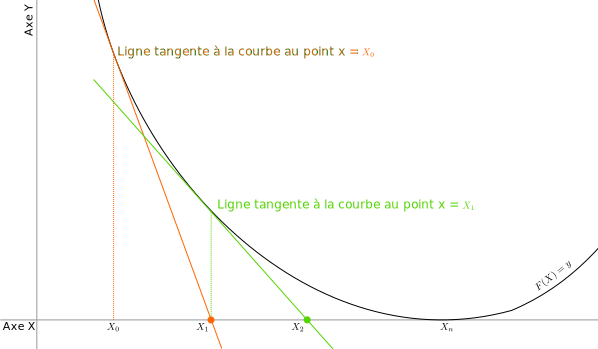
\includegraphics[width=0.8\textwidth]{newton}
  \caption{Exemple de deux étapes de Newton in une dimension.
    Chaque tangente corresponde à une équation linéaire à résoudre.
    Nous recherchons $X_n$ et nous démarrons au point $X_0$.}
\label{fig:newton}
\end{figure}

L'exemple de la figure~\ref{fig:newton} n'est que dans une seule dimension, mais la même approche peut être utilisée quand on travaille avec un nombre arbitraire de dimensions.
%
Les équations linéaires de la simulation de réservoir peuvent être représentées sous la forme d'une matrice creuse très grande.
%
Dans cette matrice, chaque ligne représente les interactions des éléments d'une cellule avec les éléments de son voisinage direct.
%
Donc, si nous prenons un cube 3D régulier, nous pouvons avoir jusqu'à sept interactions par lignes.
%
Chaque interaction est représentée sous la forme d'une petite matrice dense dont la taille correspond au nombre de variables primaires.
%
Par la suite, un solveur de systèmes d'algèbre linéaire creux est utilisé.
%
Pour la simulation de réservoir, nous utilisons un GMRES préconditionné parce que nos matrices ne sont pas symétriques.

%+++++++++++++++++++++++++++++++


%+++++++++++++++++++++++++++++++
\section{Linear algebra}
%-------------------------------
\subsection{Algèbre linéaire dense}
Résoudre un système d'équations linéaire équivaut à résoudre un problème du type $Ax=b$ dans lequel $A$ est une matrice, $b$ est le vecteur second membre du système et $x$ est le vecteur que nous cherchons.
%
Dans l'exemple de la simulation de colonne d'huile, nous avons une matrice triangulaire pour $A$, la solution peut donc être trouvée directement en résolvant chaque équation une à une en démarrant par $P(X_0) = 1000$.
%
Mais ce n'est pas toujours aussi facile.
%
Dans des cas plus difficiles, d'autres méthodes doivent être utilisées comme l'élimination de Gauss-Jordan, l'élimination de variables ou bien la décomposition LU.


En informatique, il existe plusieurs bibliothèques spécialisées dans les opérations d'algèbre linéaire dense.
%
La plus connue est BLAS\footnote{Basic Linear Algebra Subprograms}, c'est un ensemble d'opérations d'algèbre linéaire qui s'appliquent sur des vecteurs et des matrices.
%
Ces opérations sont classées en 3 niveaux :
\begin{itemize}
  \item Niveau 1 : ce sont les opérations sur les vecteurs (produit scalaire, addition de deux vecteurs, ...);
  \item Niveau 2 : ce sont les opérations matrice-vecteur (multiplier une matrice par un vecteur, résoudre un système d'équations linéaires dont les coefficients sont dans une matrice triangulaire, ...);
  \item Niveau 3 : ce sont les opérations matrice-matrice (multiplier une matrice par une autre matrice, ...).
\end{itemize}
%
Le niveau des BLAS est directement lié à leur complexité en nombre d'opérations.
%
Les BLAS de niveau 1 sont limités par la bande passante mémoire, il n'y a aucune réutilisation des données.
%
Chaque donnée n'est utilisée qu'une seule fois, la seule optimisation possible se fait au niveau du prefetch mémoire.
%
Les BLAS de niveau 2 peuvent réutiliser des données du vecteur, des optimisations peuvent être effectuées ici, par exemple il est possible de garder des parties du vecteur en cache.
%
Les BLAS de niveau 3 ont une complexité plus grande ce qui permet d'avoir un plus grand nombre d'optimisations~\cite{blas3_opt}.

LAPACK\footnote{Linear Algebra PACKage} est une autre bibliothèque utilisée en algèbre linéaire, elle est construite par dessus BLAS.
%
Les opérations faites dans BLAS et LAPACK sont bien optimisées, par exemple certaines implémentations utilisent la structuration en bloc qui permet d'optimiser la localité des données et de réduire les défauts de cache.
%
D'autres implémentations utilisent les instructions SIMD(SSE, AVX, ...) des processeurs modernes~\cite{intel_mkl}.
%
Des implémentations GPGPU\footnote{Genenal Purpose Graphical Processing Unit}~\cite{nvidia_cublas} existent aussi, de même que des implémentations en mémoire distribuée~\cite{dplasma}.
%
La plupart de ces optimisations peuvent exister parce que le motif des accès mémoires des opérations du type BLAS est déterministe et que certaines opérations peuvent être réordonnées sans impacter le résultat final.


Retournons à la matrice de l'équation~\eqref{eq:ax_b}, nous pouvons voir que cette matrice contient énormément de valeurs nulles et que ces valeurs n'ont aucun impact sur le calcul.
%
On peut différencier les matrices avec beaucoup de valeurs nulles, des matrices avec une majorité de valeurs non nulles.
%
Une matrice peut être considérée creuse quand son nombre de valeurs non nulles est de l'ordre de la dimension de la matrice.
%
Les méthodes utilisées pour résoudre les systèmes linéaires creux sont différentes de celles utilisées pour les systèmes linéaires denses.

%-------------------------------
\subsection{Algèbre linéaire creuse}
A la différence de l'algèbre linéaire dense, la majorité des calculs fait en creux sont irrégulier.
%
C'est en partie dû à la façon de stocker la matrice creux.
%
En effet, pour avoir un stockage efficace, seul les coefficients non nuls de la matrice creuse sont stockés.
%
Le motif des valeurs non nuls de la matrice est définit par le problème que nous souhaitons résoudre.
%
Le format le plus générique pour stocker des matrices creuses s'appelle COO (fig.~\ref{fig:COO}).
%
Dans ce format, chaque valeur non nuls est stocké avec ses coordonnées 2D dans la matrice.
%
Une autre format, lui aussi générique, est souvent utilisé, il s'agit du format CSR\footnote{Compress Sparse Row} (fig.~\ref{fig:CSR}).
%
Les éléments non nuls sont triés par ligne puis le tableau {\em PTR} du format de stockage nous permet de retrouver la ligne d'un élément.
%
D'autre formats moins générique existent mais nous n'en parlerons pas ici.

\begin{figure}[!ht]
     \begin{center}
        \subfigure[Exemple de matrice creuse]{%
            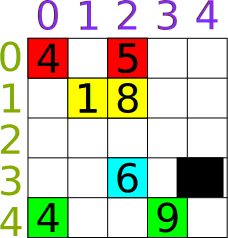
\includegraphics[width=0.25\textwidth]{matrix_format}
        }%
        \subfigure[Stockage COO]{%
           \label{fig:COO}
           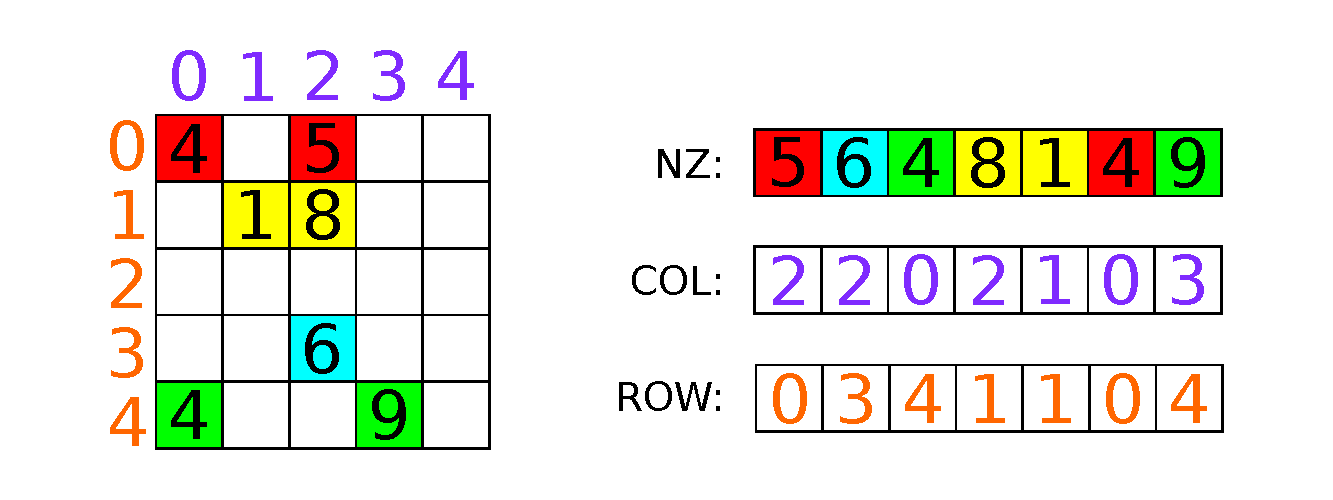
\includegraphics[width=0.35\textwidth]{COO}
        }%
        \subfigure[Stockage CSR]{%
            \label{fig:CSR}
            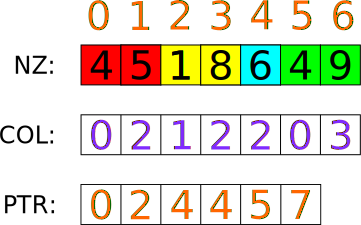
\includegraphics[width=0.35\textwidth]{CSR}
        }%
    \end{center}
    \caption{Comparaison entre les formats de stockage de matrices creuses COO and CSR.}
    \label{fig:matrix_storage}
\end{figure}

Le choix du format de stockage va avoir beaucoup d'effet sur les performances d'une application.
%
Avec la plupart des format, nous aurons au moins deux accès mémoire pour obtenir les coordonnée 2D d'un coefficient non nul alors qu'avec l'algèbre linéaire dense nous pouvons calculer ces coordonnée à partir de la position dans la matrice.
%
Une partie non négligeable de la bande passante mémoire est utilisée juste pour les coordonnée 2D.
%
Les propriétés creuse et irrégulière de ces matrices implique aussi une mauvaise efficacité mémoire des noyaux d'algèbre linéaire creux à cause d'une mauvaise réutilisation du cache.
%
La plupart des optimisations faites en algèbre linéaire dense ne peuvent pas être appliquées à l'algèbre linéaire creuse à cause de l'irrégularité dans l'ordre des calculs ainsi que dans les accès mémoire.
%
Mais l'algèbre linéaire creuse nous permet de résoudre des problèmes bien plus grand que ceux qui utilise l'algèbre linéaire dense.
%
Ceci est dû au fait qu'avec une taille de matrice équivalente, l'algèbre linéaire creuse utilise vraiment moins de mémoire que l'algèbre linéaire dense.


Résoudre des problèmes linéaire creux est aussi très différent de résoudre des problèmes denses.
%
Nous ne pouvons pas utiliser une inversion directe de matrice, ou la technique de l'élimination de Gauss parce que nous obtiendrions une matrice quasi-dense.
%
Or une matrice quasi-dense avec de grandes dimensions ne pourrait pas tenir en mémoire et même si c'était le cas, le nombre de calcul serait trop important.
%
Donc des méthodes différentes ont été inventées pour être capable de résoudre ces problèmes, beaucoup sont basées sur des méthodes itératives.
%
Nous démarrons donc avec une solution, ensuite ces algorithmes réduisent itérativement la différence entre notre solution approximée et la solution réelle.
%
A la fin, nous obtenons une bonne approximation de la solution ce qui est souvent suffisant pour être considérée comme la solution au problème.

%+++++++++++++++++++++++++++++++


%+++++++++++++++++++++++++++++++
\section{Solving large sparse linear system}
%-------------------------------
\subsection{GMRES}
  \begin{itemize}
    \item Iterative method for general matrix
    \item Doesn't work well with our matrices
  \end{itemize}
%-------------------------------
\subsection{Preconditioned GMRES}
  \begin{itemize}
    \item Need to add a ILU part which is not parallel
    \item Improve a lot convergence of our matrices
  \end{itemize}
%-------------------------------
\subsection{Domain decomposition}
  \begin{itemize}
    \item Can be use to obtain complete parallel part
    \item Degrade convergence
  \end{itemize}
%-------------------------------
\subsection{Reservoir case studies}
  \begin{itemize}
    \item SPE10, often use in reservoir benchmark
    \item generate
    \item ordering -> change preconditionner performance
  \end{itemize}
%+++++++++++++++++++++++++++++++



%+++++++++++++++++++++++++++++++
\section{Computers to target}
%-------------------------------
\subsection{SMP}
  \begin{itemize}
    \item Memory don't scale with a high number of core
  \end{itemize}
%-------------------------------
\subsection{NUMA}
  \begin{itemize}
    \item Memory scale with a high number of core
    \item Need to add some support in program to obtain performance
  \end{itemize}
%-------------------------------
\subsection{Many-core}
  \begin{itemize}
    \item Xeon phi
    \item GPU ?
    \item Too many change in program but not always performance (data transfer)
  \end{itemize}
%-------------------------------
\subsection{Our computers}
\subsubsection{Rostand}
  \begin{itemize}
    \item Bi-socket
    \item NUMA
    \item 12 Cores
    \item MPI
  \end{itemize}
\subsubsection{Manumanu}
  \begin{itemize}
    \item 20 sockets
    \item NUMA
    \item Altix UV100
    \item 160 Cores
  \end{itemize}
%+++++++++++++++++++++++++++++++

%+++++++++++++++++++++++++++++++
\section{Multi-core parallelism}
%-------------------------------
\subsection{Parallel for loop}
  \begin{itemize}
    \item OpenMP
  \end{itemize}
%-------------------------------
\subsection{Task paradigm}
  \begin{itemize}
    \item PaRSEC
    \item
  \end{itemize}
%+++++++++++++++++++++++++++++++


\subsection{Runtime}
A runtime is a piece of software used by others software to abstract part of the system.
%
There are several type of runtime.
%
Some high level programming languages use runtime, for example Java has a runtime for garbage collection.
%
Also some implementations of MPI have a runtime.
%
Task based programming also tend to have a runtime.
%
In the following part, we will focus on runtime support for task based programming.



The main interest of runtime in task based programming is to schedule tasks while respecting strict dependencies order.
%Le rôle des supports d'exécution pour la programmation en tâches est d'orchestrer la réalisation des tâches en respectant leurs dépendances.
%
These runtimes also provide a load balancing over all available hardware ressources (potentially heterogeneous) while keeping data consistency.
%Ils se chargent de la répartition des tâches sur les ressources matérielles disponibles (potentiellement hétérogènes) tout en assurant la cohérence des données.
%
Some runtime also provide memory transfer between ressources, for example between main memory and a graphical card or just between two processes.
%
These transfers could be implicit, the runtime has data knowledge, or they could be explicit, a special task.


Some runtime use schedule policy (static or dynamic) to improve load balancing.
%
But the perfect scheduler doesn't exist maybe will never exist.
%
Indeed, finding the best schedule for a set of tasks on a limited number of resources machine is a NP-complete problem\footnote{A problem is NP-complete if the solving time is polynomial compare to input data.}.
%
Some heuristic are used to obtain some reasonably good results, for example the greedy algorithm.
%
Also, some heuristic needs more information about tasks, like an estimated cost.


\subsection{Timeline of runtime}
Back in 80's, some scientist succeed in interconnecting some processors together and obtain a parallel machine,

A new idea appears to make scheduler , it's name is {\em work-stealing}.
La notion de vol de tâches (en anglais \textit{work-stealing}) apparaît ensuite, ce qui rend les ordonnanceurs dynamiques.
%
With this idea, tasks can be schedule during run-time, when a hardware resource is free.
%
One of the best example is Cilk~\cite{Cilk}, first published in 1994 and still developed under the Cilk++~\cite{Cilk++}.
%
Tasks are describe by the programmer with additional keywords to the C language, for example in Cilk the keyword {\em spawn} before a function call means that a task must be create and the runtime can schedule it.
%
In the case of Cilk a specific compiler must be use in order to transform the code into a set runtime call, this is close of source-to-source compiler.
%
The parallelism that consist in spawning tasks and then wait for some of them is often called {\em insert task} paradigm.
%
One can also used the name {\em sequential task graph} because the task graph is build along the computation.
%
On the opposite, one can found {\em Parametrized Task Graph} or in a shorter way {\em PTG} where the graph .

OpenMP~\cite{OpenMP} is a different from above, it is a runtime specialized in loop parallelism without data dependency.
%
Somewhat like Cilk, it uses some language extension ({\em \#pragma omp <action>} in C) and a specific compiler must be used to translate the code (transform the loop into a function and call the right runtime functions).
%
In 1997, the specification 3.0 of OpenMP add the keyword {\em task} to support {\em sequential task graph}, it still doesn't support implicit data dependencies.
%
More recently, the specification 4.0 add an support of implicit data dependencies.
%
To date, OpenMP is certainly the most commonly used runtime through that one can obtain a parallel application with the simple well know line {\em \#pragma omp parallel for}


At begin of 2000's, architecture in the processor became parallel.
%
Two or more cores cohabit on a single chip and share some resources like cache or memory bandwidth.
%
One can have multi threading parallelism, but there is need of runtime to exploit this parallelism.
%
For example, Intel TBB (\textit{Threading Building Blocks})~\cite{TBB} which is developed by Intel since 2006 especially for abstract multi-core programming and with the same goal SMPSs~\cite{SMPSs}(now part of STARSs, see below) since 2007.

When we use a cluster, there is two choice.
%
On the one hand, there is DSM\footnote{Distributed Shared Memory}, which is very simple to use but
%
On the other hand, there is message passing paradigm, which is more difficult to use but give good result.
%
It is the most used paradigm for distributed memory especially with the MPI norm.
%

More recently, in the late 2000's, the GPGPU revolution leads the apparition of new type of runtime.
%
These runtimes must now support heterogeneous resources with sometimes several address spaces.
%
They must also integrate a support to automatically transfer data between the several address space.
%
Among these runtimes, one can found StarPU~\cite{ATNW2011,Aug2011}, PaRSEC~\cite{PaRSEC} (formerly called DAGuE~\cite{DAGuE2012}), X-KAAPI~\cite{X-KAAPI} and STARSs (became OMPSs~\cite{OMPSs} by the merge of SMPSs, ClusterSs and CellSs,\dots).

Some runtime specialized in loop parallelism also gain a GPU support, like OpenMP in is specification 4.0.
%
But this specification is mostly inspired from OpenACC~\cite{OpenACC} which wants to simplify parallel programming of heterogeneous CPU/GPU systems.

Meanwhile, Intel prepare a against GPU, the {\em Kinghts Corner}.
%
A PCI express card with around 60 cores with the well known architecture x86, more precisly an old pentium architecture with a very powerful SIMD unit.
%
The main advantage of this architecture, is that the card can be seen as a computer with 60 cores totally independent because a standard kernel can run inside.
%
So almost all runtime are directly compatible or just need minor changes.



\subsection{Classification of runtime}
We can try to classify all these runtime by functionality, we can consider three form of parallelism expression : loop parallelism, PTG and insert task paradigm.
%
The first table~\ref{tab:runtime_family} summarizes capabilities of a set of runtime, a {\it ++} entry means that the capacity is often put forward in publication, a single {\it +} means that the runtime has the functionality but it is not a major advantage of the runtime.
%
The second table~\ref{tab:runtime_archi} summarizes target architecture of the same set of runtime.
%
In the case of distributed memory, we can see two method to address this problem.
An implicit method when the runtime has a memory manager and can do automatic transfer.
Or an explicit method often describe as user task, some runtime, like StarPU, support asynchronous transfer, without this support the explicit method is less efficient.


We can also try to differentiate other differences, like the use of an API ({\it Application Programming Interface}) or the use of a source-to-source compiler.
%
Data management is also important in a runtime to optimize data transfer between CPU and GPU, or between two CPUs.

\begin{table}[h!]
\centering
\begin{tabular}{c|ccc}
  \textit{runtime}& loop parallelism & PTG & Insert task\\
  \hline
        Cilk           &    &    & ++ \\
        Cilk++         & ++ &    & ++ \\
        OpenMP $<$ 3.0 & ++ &    &    \\
        OpenMP 3.x     & ++ &    & +  \\
        OpenMP 4.0     & ++ &    & +  \\
        OpenACC        & ++ &    & +  \\
        Intel TBB      & +  &    & ++ \\
        OMPSs          & +  &    & ++ \\
        Intel CnC      & +  & ++ &    \\
        PaRSEC         &    & ++ &    \\
 PGAS(coarray fortran) & ++ &    &    \\
        StarPU         &    &    & ++ \\
        KAAPI          & ++ &    &    \\
        X-KAAPI        & +  &    & ++
\end{tabular}
\caption{Classification of runtime by capabilities}
\label{tab:runtime_family}
\end{table}

\begin{table}[h!]
\centering
\begin{tabular}{c|ccc}
  \textit{runtime} & Shared memory & Distributed memory & GPU accelerator \\
\hline
        Cilk           & X &           &   \\
        Cilk++         & X &           &   \\
        OpenMP $<$ 3.0 & X &           &   \\
        OpenMP 3.x     & X &           &   \\
        OpenMP 4.0     & X &           & X \\
        OpenACC        & X &           & X \\
        Intel TBB      & X &           &   \\
        OMPSs          & X & explicit  & X \\
        Intel CnC      & X & implicit  &   \\
        PaRSEC         & X & implicit  &   \\
 PGAS(coarray fortran) & X & implicit  &   \\
        StarPU         & X & implicit/explicit  & X \\
        KAAPI          & X &           & X \\
        X-KAAPI        & X & explicit  & X
\end{tabular}
\caption{Classification of runtime by supported architecture}
\label{tab:runtime_archi}
\end{table}





%=========================================================
\chapter{A problem of granularity}
\minitoc
\vspace{1cm}
%=========================================================
%+++++++++++++++++++++++++++++++
\section{Parallelize preconditioned GMRES}
%-------------------------------
\subsection{GMRES algorithm}
  \begin{itemize}
    \item Explain GMRES algorithm
    \item it is mostly parallel for BLAS1 and BLAS2
    \item We need to use a preconditionner
  \end{itemize}
%-------------------------------
\subsection{Incomplete LU}
LU factorization in dense linear algebra is a method to factorize a matrix $A$ into two matrices $L$ and $U$.
%
$L$ is a triangular lower matrix, all value above the diagonal are zeros.
%
Same thing for $U$, but all zeros are under the diagonal.
%
The main interest of this factorization is to solve x in the equation of type $A.x=y$.
%
This equation is transform into two equations $L.x_{tmp}=y$ and $U.x=x_{tmp}$.
%
Solving a system with a triangular matrix is pretty trivial.
%
This can be done row by row by starting by the row with only one value.
%
Then the row with two values can solve and so on.
%
This algorithm is purely sequential but some works exist to make it parallel %TODO ref sur plasma

In sparse linear algebra, we can't do exact LU factorization because it will result two dense matrices $L$ and $U$.
%
So we use an alterate form of LU which is ILU (Incomplete LU).
%
The ILU algorithm is quite the same as LU but the non-zero patern of the matrix $A$ is the same as non-zero patern of matrices $L$ and $U$.
%
The parallelism in ILU naturally exists, some rows can be factorize in parallel.
%
To factorize a specific row we need to look at it non-zero pattern.
%
The indices of all non-zeros before the diagonal give us the list of rows that need to factorize first. %TODO figure
%
The parallelism can be represent under a DAG form. %TODO figure

So, the parallelism in ILU can be represent under a task form.
%
Each task represents the factorization of one row... which is quite small.
%
In fact, most of task scheduler will take longer to schedule the task than the task takes to factorize a row.
%
It's called granularity problem.
%
To solve this problem, tasks must become bigger.
%
To do that, we can factorize several rows in one task.
%
But it is not simple to choice which tasks could be factorized together without impacting result or parallelism.
%
A generic method is shown later in this thesis.

%-------------------------------
%+++++++++++++++++++++++++++++++

%+++++++++++++++++++++++++++++++
\section{Why granularity is so important ?}
%-------------------------------
\subsection{Parallelism vs overhead}
  \begin{itemize}
    \item Talk about runtime overhead
    \item Give some result without aggregation
  \end{itemize}
%-------------------------------
\subsection{Current solutions}
  \begin{itemize}
    \item X-KAAPI
    \item SCOOP
    \item Capsules
    \item for each explain why they don't fit our problem
  \end{itemize}
%+++++++++++++++++++++++++++++++


%+++++++++++++++++++++++++++++++
\section{My solution to our granularity problem}
%-------------------------------
\subsection{Taggre : a task aggregator framework}
%-------------------------------
\subsection{Aggregate operators}
  \begin{itemize}
    \item Put tasks together without making cycle in DAG
  \end{itemize}
%-------------------------------
\subsubsection{Sequential}
\subsubsection{Front}
\subsubsection{Depth front}
\subsubsection{Continuation oriented}
%-------------------------------
\subsection{Examples of strategies}
  \begin{itemize}
    \item Talk about the 7 dwarfs (\url{http://view.eecs.berkeley.edu/wiki/Dwarf_Mine})
  \end{itemize}
%+++++++++++++++++++++++++++++++




%+++++++++++++++++++++++++++++++
\section{Results}
%-------------------------------
\subsection{Factorization and Triangular solve improvement}
  \begin{itemize}
    \item Explain why we benchmark this part
    \item Try a lot of coarse string
  \end{itemize}
%-------------------------------
\subsection{Aggregation overhead}
  \begin{itemize}
    \item Explain why it isn't a real problem
    \item Give some numbers
  \end{itemize}
%-------------------------------
\subsection{Subdomain decomposition}
  \begin{itemize}
    \item Explain why it isn't a real problem
    \item Give some numbers
    \item Talk about bandwidth
  \end{itemize}
%-------------------------------
\subsection{Discussion}
  \begin{itemize}
    \item Compare domain with domain decomposition
  \end{itemize}
%+++++++++++++++++++++++++++++++





%=========================================================
\chapter{Memory bandwidth limitation}
\minitoc
\vspace{1cm}
%=========================================================
%+++++++++++++++++++++++++++++++
\section{Pourquoi mon SpMV est si lent ?}
%-------------------------------
\subsection{Deux fois plus de coeurs mais pas deux fois plus rapide}
  \begin{itemize}
    \item Just draw some curves
  \end{itemize}
%-------------------------------
\subsection{Explication de la mémoire}
Pour comprendre les résultats précédent nous devons étudier brièvement l'architecture des ordinateurs.
%
Les performances d'un ordinateur dépendent essentiellement de deux choses : le processeur et la mémoire.
%
Quand un programme souhaite lire une donnée en mémoire, il subit une pénalité mémoire.
%
Cette pénalité est la somme de deux contraintes :
\begin{itemize}
        \item la latence : la différence de temps entre la demande d'accès à la mémoire et la réception du premier octet;
        \item la bande passante : le nombre maximum d'octet par seconde que le bus peut envoyer/recevoir
\end{itemize}
%
In a modern computer, there is different type of memories.
%




  \begin{itemize}
    \item Define memory penalty
    \item Talk about bandwidth
  \end{itemize}
%+++++++++++++++++++++++++++++++

De manière générale, quand un programme alloue de la mémoire, il reçoit un pointeur sur de la mémoire virtuelle.
%
Cette mémoire virtuelle est unique à chaque processus et est partagée entre les threads.
%
La relation entre la mémoire virtuelle et la mémoire physique est faite par le système d'exploitation.
%
Il est en charge de la bonne gestion de la mémoire physique.
%
Lorsqu'un processus accède à de la mémoire virtuelle qui n'as pas encore été mappée à de la mémoire physique, une faute de page est générée, on appelle ça toucher une page.
%
Cette faute est traitée par le système d'exploitation, il s'occupera de trouver une page mémoire libre dans la mémoire physique et il la fera correspondre à une adresse virtuelle.
%
Lors des accès mémoire du processus, la translation de l'adresse virtuelle vers l'adresse physique est faite par un des composant du processeur, l'unité de gestion mémoire ou MMU\footnote{Memory Management Unit}.
%
De cette façon, le processus ne voit que l'espace d'adressage virtuelle et ne connaît rien de l'espace d'adressage physique.
%
Le système d'exploitation peut donc changer l'emplacement physique d'une page sans affecter le fonctionnement du processus, c'est totalement transparent.
%
Toutefois, l'emplacement physique d'une page virtuelle peut impacter les performance du processus sur les architectures NUMA.
%
Cet impact dépendra des connexions entre le banc mémoire physique où se situe la page et le coeur de calcul qui fait tourner le processus.


Sur une machine NUMA, lorsqu'une faute de page arrive, le système d'exploitation doit choisir sur quel banc NUMA il placera la page.
%
Avec Linux, il y a au moins trois politiques d'allocations de disponibles :
\begin{itemize}
        \item {\em First Touch}: La mémoire est allouée sur le banc NUMA du coeur de calcul qui y accède en premier.
                         Il s'agit de la politique par défaut.
        \item {\em Bind}: La mémoire est allouée sur banc NUMA spécifié en paramètre.
        \item {\em Interleaved}: Les allocations mémoire sont entrelacées parmi tous les bancs NUMA disponibles.
\end{itemize}
Sur Linux, ces politiques peuvent être choisies avec l'appel système {\em mbind}, ou avec l'outil en ligne de commande {\em numactl}.
%
La version 3.13 de Linux apporte un nouveau mécanisme de gestion de la mémoire sur les machine NUMA, il s'agit d'AutoNUMA.
%
Ce mécanisme a pour but d'optimiser le placement des pages NUMA tout long de l'exécution d'un processus (Voir section~\ref{sec:autonuma}).


D'autres système d'exploitation peuvent avoir leurs propres ensembles de politiques d'allocations NUMA.
%
Solaris, par exemple, fournit aussi la politique {\em next-touch}~\cite{next_touch}.
%
Avec cette politique, les pages mémoires physique seront déplacées près du prochain coeur de calcul qui y accédera (Voir section~\ref{sec:next_touch}).


%+++++++++++++++++++++++++++++++
\section{Handle NUMA directly in scheduler}
%-------------------------------
\subsection{Status of current scheduler}
  \begin{itemize}
    \item PaRSEC : one vp per NUMA
  \end{itemize}
%-------------------------------
\subsection{NATaS : schedule tasks on NUMA}
  \begin{itemize}
    \item bind task to a processor
    \item allow NUMA work-stealing
    \item bind memory pages
  \end{itemize}
%+++++++++++++++++++++++++++++++


%+++++++++++++++++++++++++++++++
\section{Results}
%-------------------------------
\subsection{Factorization and Triangular solve}
  \begin{itemize}
    \item Support NUMA in tasks
  \end{itemize}
%-------------------------------
\subsection{Sparse matrix vector multiplication}
  \begin{itemize}
    \item problem of SpMV
  \end{itemize}
%-------------------------------
\subsection{First touch}
results
%-------------------------------
\subsection{Interleave}
results
%-------------------------------
\subsection{Automatic NUMA balancing}
  \begin{itemize}
    \item Results on personal machine
    \item very recent kernel
  \end{itemize}
%-------------------------------
\subsection{NATaS}
results
%-------------------------------
\subsection{Discussion}
  \begin{itemize}
    \item Interleave isn't so bad on bi-socket,...
    \item NATaS always give best result
    \item Maybe NATaS isn't the good answer (better scheduler or MPI)
  \end{itemize}
%+++++++++++++++++++++++++++++++


%=========================================================
\chapter{The fork and join syndrome}
\minitoc
\vspace{1cm}
%=========================================================
%+++++++++++++++++++++++++++++++
%\section{Data dependencies}
%-------------------------------
%\subsection{Implicit dependencies}
%-------------------------------
%\subsection{Explicit dependencies}
%+++++++++++++++++++++++++++++++


%+++++++++++++++++++++++++++++++
\section{The fork and join syndrome}
%-------------------------------
\subsection{How to see it ?}
  \begin{itemize}
    \item Show that we have too much synchronization (Paje trace)
  \end{itemize}
%-------------------------------
\subsection{Domain decomposition and overlap}
  \begin{itemize}
    \item Explain what domain decomposition and overlap is
  \end{itemize}
%+++++++++++++++++++++++++++++++


%+++++++++++++++++++++++++++++++
\section{Pipeline GMRES steps}
  \begin{itemize}
    \item explain the solution to merge graph of task
  \end{itemize}
%+++++++++++++++++++++++++++++++


%+++++++++++++++++++++++++++++++
\section{Results}
%-------------------------------
\subsection{Without MPI}
  \begin{itemize}
    \item Almost no gain because no many sync
  \end{itemize}
%-------------------------------
\subsection{With MPI}
  \begin{itemize}
    \item Gain when increase number of MPI process
  \end{itemize}
%-------------------------------
\subsection{Discussion}
%+++++++++++++++++++++++++++++++




%=========================================================
\chapter{Conclusions and perspectives}
\minitoc
\vspace{1cm}
%=========================================================
%+++++++++++++++++++++++++++++++
\section{Conclusion}
  \begin{itemize}
    \item Coarsening allow us to parallelize problems with very small computation per task
    \item Improve bandwidth thanks to NUMA architecture
  \end{itemize}
%+++++++++++++++++++++++++++++++


%+++++++++++++++++++++++++++++++
\section{Perspectives}
  \begin{itemize}
    \item Automatic coarse tuning
  \end{itemize}
%+++++++++++++++++++++++++++++++



\backmatter % book mode only
%\bibliographystyle{alpha}
%\bibliography{anrt}
\appendix

\bibliographystyle{plainnat}
\bibliography{thesis}
\end{document}
